%% GENERATED by tools/from_docs.py from stepss-docs. Do not edit by hand:
%% edit the page named below in stepss-docs and regenerate.
%% source: stepss-docs/src/content/docs/models/exciters/ieee-ac-dc.md

\chapter{IEEE AC and DC exciters}\label{doc:model-exc-ieee-acdc}

The rotating-exciter models of IEEE Std 421.5 available in RAMSES: three alternator-supplied (AC) types and one DC type.

The \texttt{EXC} sub-record these models are entered with, and the table of IEEE model variants, are on the \hyperref[doc:model-exc]{Exciter Models} page.

\section{AC1A}\label{model-exc-ieee-acdc:ac1a}

The AC1A is a rotating AC exciter with a self-excited field winding and non-linear saturation. It corresponds to IEEE Std 421.5-2016 Type AC1A. The generator terminal voltage \(V_t\) is compensated for line drop and filtered before being compared with the reference. An AC alternator supplies the field through a rectifier whose output depends on the commutation voltage \(V_E\) and field current \(I_{fd}\).

\begin{figure}[htbp]
\centering
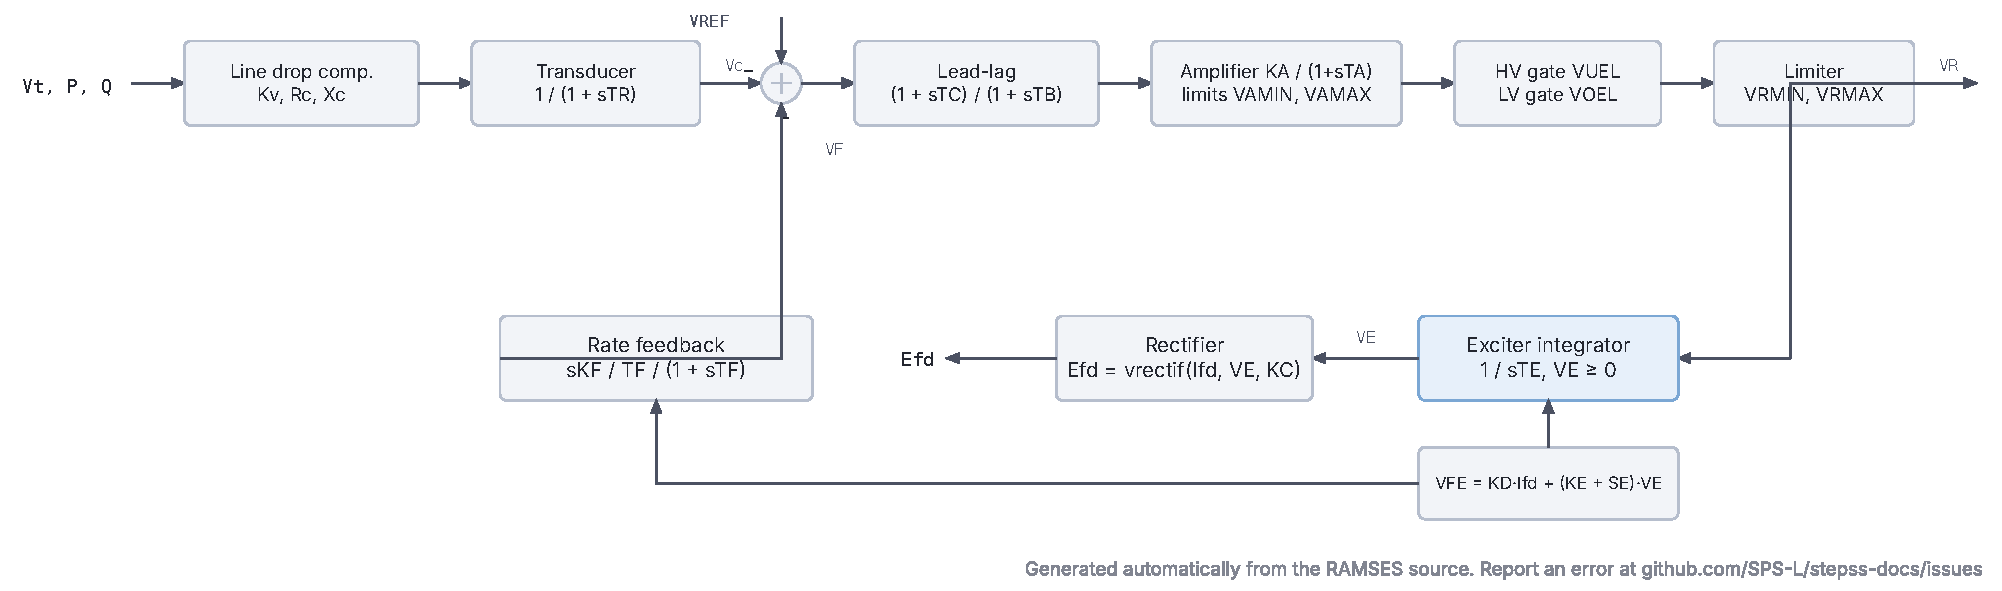
\includegraphics[width=0.98\linewidth]{figures/exc-ac1a-light}
\caption{AC1A block diagram.}
\end{figure}

\subsection{Mathematical Description}\label{model-exc-ieee-acdc:mathematical-description}

The voltage regulator processes the error signal through a lead-lag network and a limited amplifier:

\[\Delta V = V_{REF} - V_c - V_F - \Delta V_{PSS}\]

\[V_1(s) = \Delta V \cdot \frac{1 + sT_C}{1 + sT_B}\]

\[V_A(s) = V_1 \cdot \frac{K_A}{1 + sT_A}, \quad V_{AMIN} \le V_A \le V_{AMAX}\]

The AC exciter integrator with saturation and demagnetization:

\[V_{FE} = K_D \cdot I_{fd} + \left(K_E + S_E(V_E)\right) V_E\]

\[\dot{V}_E = \frac{1}{T_E}(V_R - V_{FE}), \quad 0 \le V_E\]

\[E_{fd} = V_E \cdot \left(1 - \frac{K_C \cdot I_{fd}}{V_E}\right)\]

The derivative feedback (rate feedback) path:

\[V_F(s) = E_{fd} \cdot \frac{sK_F/T_F}{1 + sT_F}\]

where \(S_E(V_E)\) is the saturation function interpolated from the two-point saturation characteristic \((V_{E1}, SE_1)\) and \((V_{E2}, SE_2)\).

\subsection{Signal Flow}\label{model-exc-ieee-acdc:signal-flow}

\begin{enumerate}
\def\labelenumi{\arabic{enumi}.}
\tightlist
\item
  \textbf{Line drop compensation} (\texttt{algeq}): \(V_{c1} = vcomp(V_t, P, Q, K_v, R_c, X_c)\)
\item
  \textbf{Voltage measurement filter} (\texttt{tf1p}): \(V_c \leftarrow V_{c1}\) with time constant \(T_R\)
\item
  \textbf{AVR summation} (\texttt{algeq}): \(\Delta V = V_{REF} - V_c - V_F\)
\item
  \textbf{Lead-lag compensator} (\texttt{tf1p1z}): \(V_1 \leftarrow \Delta V\) with \((T_C, T_B)\)
\item
  \textbf{Amplifier with limits} (\texttt{tf1plim}): \(V_2 \leftarrow V_1\) with gain \(K_A\), time constant \(T_A\), limits \([V_{AMIN}, V_{AMAX}]\)
\item
  \textbf{UEL high-value gate} (\texttt{max1v1c}): \(V_3 = \max(V_2, V_{UEL})\)
\item
  \textbf{OEL low-value gate} (\texttt{min1v1c}): \(V_4 = \min(V_3, V_{OEL})\)
\item
  \textbf{Output limiter} (\texttt{lim}): \(V_R = \text{clamp}(V_4, V_{RMIN}, V_{RMAX})\)
\item
  \textbf{Exciter integrator} (\texttt{inlim}): \(V_E \leftarrow (V_R - V_{FE})/T_E\)
\item
  \textbf{Saturation computation} (\texttt{algeq}): \(V_{FE}\) from \(K_D\), \(K_E\), \(S_E(V_E)\)
\item
  \textbf{Rectifier output} (\texttt{algeq}): \(E_{fd} = vrectif(I_{fd}, V_E, K_C)\)
\item
  \textbf{Derivative feedback} (\texttt{tfder1p}): \(V_F \leftarrow V_{FE}\) with gain \(K_F/T_F\), time constant \(T_F\)
\end{enumerate}

\subsection{Parameters}\label{model-exc-ieee-acdc:parameters}

\begin{small}\begin{longtable}[]{@{}lll@{}}
\toprule\noalign{}
Parameter & Description & Unit/Type \\
\midrule\noalign{}
\endhead
\bottomrule\noalign{}
\endlastfoot
\texttt{Kv} & Voltage compensation gain & pu \\
\texttt{Rc} & Resistance for line drop compensation & pu \\
\texttt{Xc} & Reactance for line drop compensation & pu \\
\texttt{TR} & Voltage transducer time constant & s \\
\texttt{KA} & Voltage regulator gain & pu \\
\texttt{TA} & Voltage regulator time constant & s \\
\texttt{TB} & Lead-lag denominator time constant & s \\
\texttt{TC} & Lead-lag numerator time constant & s \\
\texttt{VAMAX} & Maximum regulator output & pu \\
\texttt{VAMIN} & Minimum regulator output & pu \\
\texttt{KE} & Exciter constant (self-excitation term) & pu \\
\texttt{TE} & Exciter time constant & s \\
\texttt{KF} & Rate feedback gain & pu \\
\texttt{TF} & Rate feedback time constant & s \\
\texttt{VRMAX} & Maximum field voltage & pu \\
\texttt{VRMIN} & Minimum field voltage & pu \\
\texttt{VE1} & Saturation factor voltage point 1 & pu \\
\texttt{SE1} & Saturation factor at \(V_{E1}\) & pu \\
\texttt{VE2} & Saturation factor voltage point 2 & pu \\
\texttt{SE2} & Saturation factor at \(V_{E2}\) & pu \\
\texttt{KC} & Commutation factor (rectifier regulation) & pu \\
\texttt{KD} & Demagnetization factor & pu \\
\texttt{VUEL} & UEL input signal & pu \\
\end{longtable}\end{small}

\subsection{Variants}\label{model-exc-ieee-acdc:variants}

\begin{small}\begin{longtable}[]{@{}
  >{\raggedright\arraybackslash}p{(\linewidth - 4\tabcolsep) * \real{0.2937}}
  >{\raggedright\arraybackslash}p{(\linewidth - 4\tabcolsep) * \real{0.7063}}
@{}}
\toprule\noalign{}
\begin{minipage}[b]{\linewidth}\raggedright
Model
\end{minipage} & \begin{minipage}[b]{\linewidth}\raggedright
Description
\end{minipage} \\
\midrule\noalign{}
\endhead
\bottomrule\noalign{}
\endlastfoot
\texttt{AC1A} & Base model, IEEE Type AC1A \\
\texttt{AC1A\_MAXEX2} & Adds MAXEX2 field current limiter; VOEL moves to reference summation point (LV gate removed) \\
\texttt{AC1A\_RETRO} & Retrofit variant with internal PSS4B; uses first-order AVR without separate exciter block \\
\texttt{AC1A\_RETRO\_PSS4B} & Retrofit variant with external PSS4B speed input \\
\end{longtable}\end{small}

\subsection{Usage Example}\label{model-exc-ieee-acdc:usage-example}

\begin{Verbatim}
SYNC_MACH  g1  g1
      # FP FQ P Q: share of the power-flow injection (FP, FQ) or initial power (P in MW, Q in Mvar)
      1.  1.  0.  0.
      # SNOM: Nominal apparent power, used as base power in the machine model (MVA)
      800.
      # Pnom: Nominal active power of the turbine, used as base power for the turbine model (MW)
      760.
      # H: Inertia constant (s)
      3.
      # D: Damping coefficient (usually set to zero when the damper windings are modelled) (pu)
      0.
      # IBRATIO: Field current base ratio I_fB^mac/I_fB^exc (see above) (pu)
      0.95
      # TYPE_MOD: Parameter format keyword: RL or XT (case-insensitive)
      XT
      # Xl: Leakage reactance L_l (pu)
      0.15
      # Xd: d-axis synchronous reactance (pu)
      1.1
      # X'd: d-axis transient reactance (must be smaller than Xd) (pu)
      0.25
      # X"d: d-axis subtransient reactance (pu)
      0.2
      # Xq: q-axis synchronous reactance (pu)
      0.7
      # X'q: q-axis transient reactance (pu)
      *
      # X"q: q-axis subtransient reactance (pu)
      0.2
      # m: Saturation coefficient (set to 0 to neglect saturation)
      0.1
      # n: Saturation exponent (ignored when m = 0)
      6.0257
      # Ra: Armature resistance (pu)
      0.
      # T'do: d-axis open-circuit transient time constant (s)
      5.00
      # T"do: d-axis open-circuit subtransient time constant (s)
      0.05
      # T'qo: q-axis open-circuit transient time constant (s)
      *
      # T"qo: q-axis open-circuit subtransient time constant (s)
      0.1
EXC  AC1A
      # Kv: weight of the terminal voltage in the measured voltage |Kv V + (Rc+jXc) I|; 1 = terminal voltage
      1.
      # Rc: Resistance for line drop compensation
      0.
      # Xc: Reactance for line drop compensation
      0.
      # TR: Voltage transducer time constant
      0.02
      # KA: Voltage regulator gain
      200.0
      # TA: Voltage regulator time constant
      0.02
      # TB: Lead-lag denominator time constant
      10.0
      # TC: Lead-lag numerator time constant
      1.0
      # VAMAX: Maximum regulator output
      7.32
      # VAMIN: Minimum regulator output
      -7.32
      # KE: Exciter constant (self-excitation term)
      1.0
      # TE: Exciter time constant
      1.0
      # KF: Rate feedback gain
      0.03
      # TF: Rate feedback time constant
      1.0
      # VRMAX: upper limit of the regulator output after the UEL and OEL gates (pu)
      6.03
      # VRMIN: lower limit of the regulator output after the UEL and OEL gates (pu)
      -5.43
      # VE1: Saturation factor voltage point 1
      4.18
      # SE1: Saturation factor at V_E1
      0.1
      # VE2: Saturation factor voltage point 2
      3.14
      # SE2: Saturation factor at V_E2
      0.033
      # KC: Commutation factor (rectifier regulation)
      0.2
      # KD: Demagnetization factor
      0.38
      # VUEL: UEL signal into the high-value gate; a large negative value disables it (pu)
      -99999
TOR  CONSTANT
;
\end{Verbatim}

\begin{center}\rule{0.5\linewidth}{0.5pt}\end{center}

\section{AC4A}\label{model-exc-ieee-acdc:ac4a}

The AC4A is a simplified static representation of an AC exciter system with an inner-loop voltage-dependent output limit. It corresponds to IEEE Std 421.5-2016 Type AC4A. The upper output limit is a function of field current: \(V_{RMAX,eff} = V_{RMAX} - K_C \cdot I_{fd}\).

\begin{figure}[htbp]
\centering
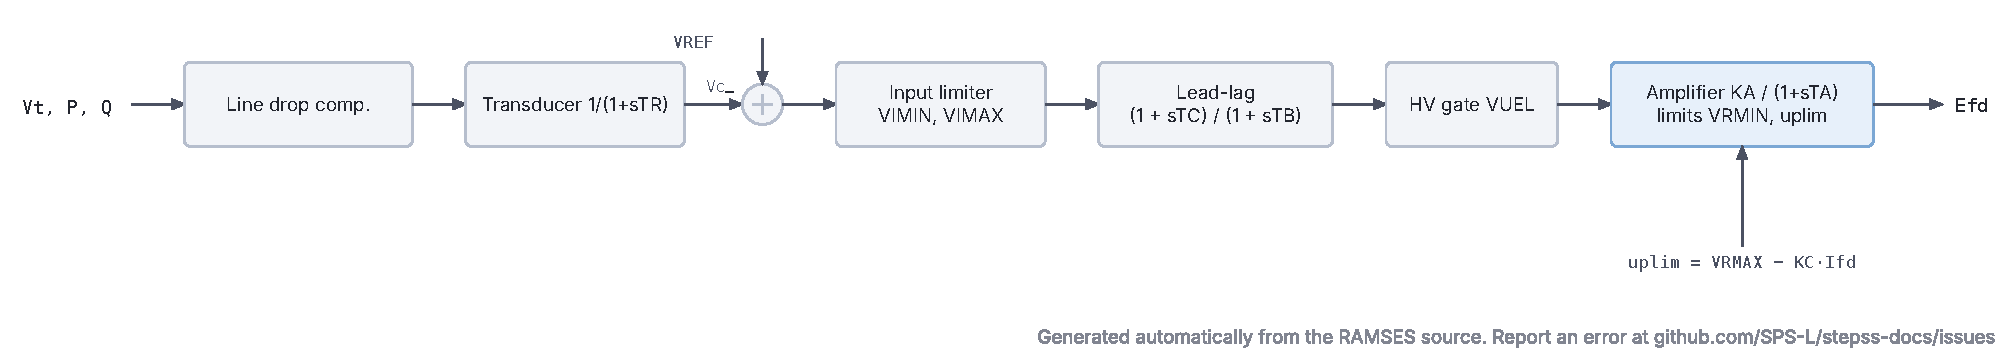
\includegraphics[width=0.98\linewidth]{figures/exc-ac4a-light}
\caption{AC4A block diagram.}
\end{figure}

\subsection{Mathematical Description}\label{model-exc-ieee-acdc:mathematical-description-1}

\[\Delta V = V_{REF} - V_c\]

\[V_I = \text{clamp}(\Delta V, V_{IMIN}, V_{IMAX})\]

\[V_1(s) = V_I \cdot \frac{1 + sT_C}{1 + sT_B}\]

\[E_{fd}(s) = V_1 \cdot \frac{K_A}{1 + sT_A}, \quad V_{RMIN} \le E_{fd} \le V_{RMAX} - K_C \cdot I_{fd}\]

The variable upper limit is updated algebraically at each time step, making AC4A a time-varying limited integrator system.

\subsection{Signal Flow}\label{model-exc-ieee-acdc:signal-flow-1}

\begin{enumerate}
\def\labelenumi{\arabic{enumi}.}
\tightlist
\item
  \textbf{Line drop compensation} (\texttt{algeq}): \(V_{c1}\) from terminal measurements
\item
  \textbf{Voltage measurement filter} (\texttt{tf1p}): \(V_c\) with \(T_R\)
\item
  \textbf{AVR summation} (\texttt{algeq}): \(\Delta V = V_{REF} - V_c\)
\item
  \textbf{Input limiter} (\texttt{lim}): \(V_I = \text{clamp}(\Delta V, V_{IMIN}, V_{IMAX})\)
\item
  \textbf{Lead-lag} (\texttt{tf1p1z}): \(V_1 \leftarrow V_I\) with \((T_C, T_B)\)
\item
  \textbf{UEL high-value gate} (\texttt{max1v1c}): \(V_2 = \max(V_1, V_{UEL})\)
\item
  \textbf{Variable upper limit} (\texttt{algeq}): \(uplim = V_{RMAX} - K_C \cdot I_{fd}\)
\item
  \textbf{Variable-limit amplifier} (\texttt{tf1pvlim}): \(E_{fd} \leftarrow V_2\) with \(K_A\), \(T_A\), limits \([V_{RMIN}, uplim]\)
\end{enumerate}

\subsection{Parameters}\label{model-exc-ieee-acdc:parameters-1}

\begin{small}\begin{longtable}[]{@{}lll@{}}
\toprule\noalign{}
Parameter & Description & Unit/Type \\
\midrule\noalign{}
\endhead
\bottomrule\noalign{}
\endlastfoot
\texttt{Kv} & Voltage compensation gain & pu \\
\texttt{Rc} & Line drop compensation resistance & pu \\
\texttt{Xc} & Line drop compensation reactance & pu \\
\texttt{TR} & Measurement filter time constant & s \\
\texttt{VIMAX} & Maximum input error signal & pu \\
\texttt{VIMIN} & Minimum input error signal & pu \\
\texttt{TC} & Lead numerator time constant & s \\
\texttt{TB} & Lag denominator time constant & s \\
\texttt{VUEL} & UEL signal value & pu \\
\texttt{KA} & Regulator gain & pu \\
\texttt{TA} & Regulator time constant & s \\
\texttt{VRMAX} & Maximum output (at zero field current) & pu \\
\texttt{VRMIN} & Minimum output & pu \\
\texttt{KC} & Field current derating factor & pu \\
\end{longtable}\end{small}

\subsection{Variants}\label{model-exc-ieee-acdc:variants-1}

\begin{small}\begin{longtable}[]{@{}ll@{}}
\toprule\noalign{}
Model & Description \\
\midrule\noalign{}
\endhead
\bottomrule\noalign{}
\endlastfoot
\texttt{AC4A} & Base model, IEEE Type AC4A, no PSS or OEL \\
\end{longtable}\end{small}

\subsection{Usage Example}\label{model-exc-ieee-acdc:usage-example-1}

\begin{Verbatim}
SYNC_MACH  g1  g1
      # FP FQ P Q: share of the power-flow injection (FP, FQ) or initial power (P in MW, Q in Mvar)
      1.  1.  0.  0.
      # SNOM: Nominal apparent power, used as base power in the machine model (MVA)
      800.
      # Pnom: Nominal active power of the turbine, used as base power for the turbine model (MW)
      760.
      # H: Inertia constant (s)
      3.
      # D: Damping coefficient (usually set to zero when the damper windings are modelled) (pu)
      0.
      # IBRATIO: Field current base ratio I_fB^mac/I_fB^exc (see above) (pu)
      0.95
      # TYPE_MOD: Parameter format keyword: RL or XT (case-insensitive)
      XT
      # Xl: Leakage reactance L_l (pu)
      0.15
      # Xd: d-axis synchronous reactance (pu)
      1.1
      # X'd: d-axis transient reactance (must be smaller than Xd) (pu)
      0.25
      # X"d: d-axis subtransient reactance (pu)
      0.2
      # Xq: q-axis synchronous reactance (pu)
      0.7
      # X'q: q-axis transient reactance (pu)
      *
      # X"q: q-axis subtransient reactance (pu)
      0.2
      # m: Saturation coefficient (set to 0 to neglect saturation)
      0.1
      # n: Saturation exponent (ignored when m = 0)
      6.0257
      # Ra: Armature resistance (pu)
      0.
      # T'do: d-axis open-circuit transient time constant (s)
      5.00
      # T"do: d-axis open-circuit subtransient time constant (s)
      0.05
      # T'qo: q-axis open-circuit transient time constant (s)
      *
      # T"qo: q-axis open-circuit subtransient time constant (s)
      0.1
EXC  AC4A
      # Kv: weight of the terminal voltage in the measured voltage |Kv V + (Rc+jXc) I|; 1 = terminal voltage
      1.
      # Rc: Line drop compensation resistance
      0.
      # Xc: Line drop compensation reactance
      0.
      # TR: Measurement filter time constant
      0.02
      # VIMAX: Maximum input error signal
      8.0
      # VIMIN: Minimum input error signal
      -8.0
      # TC: Lead numerator time constant
      1.0
      # TB: Lag denominator time constant
      10.0
      # VUEL: UEL signal into the high-value gate; a large negative value disables it (pu)
      -99999
      # KA: Regulator gain
      200.0
      # TA: Regulator time constant
      0.015
      # VRMAX: Maximum output (at zero field current)
      4.44
      # VRMIN: Minimum output
      -4.44
      # KC: Field current derating factor
      0.0
TOR  CONSTANT
;
\end{Verbatim}

\begin{center}\rule{0.5\linewidth}{0.5pt}\end{center}

\section{AC8B}\label{model-exc-ieee-acdc:ac8b}

The AC8B is a rotating AC exciter with a PID voltage regulator (rather than the proportional-integral amplifier of earlier types). It corresponds to IEEE Std 421.5-2016 Type AC8B. The PID structure, proportional gain \(K_{PR}\), integral gain \(K_{IR}\), and derivative gain \(K_{DR}\), provides improved transient response compared to Type AC1A.

\begin{figure}[htbp]
\centering
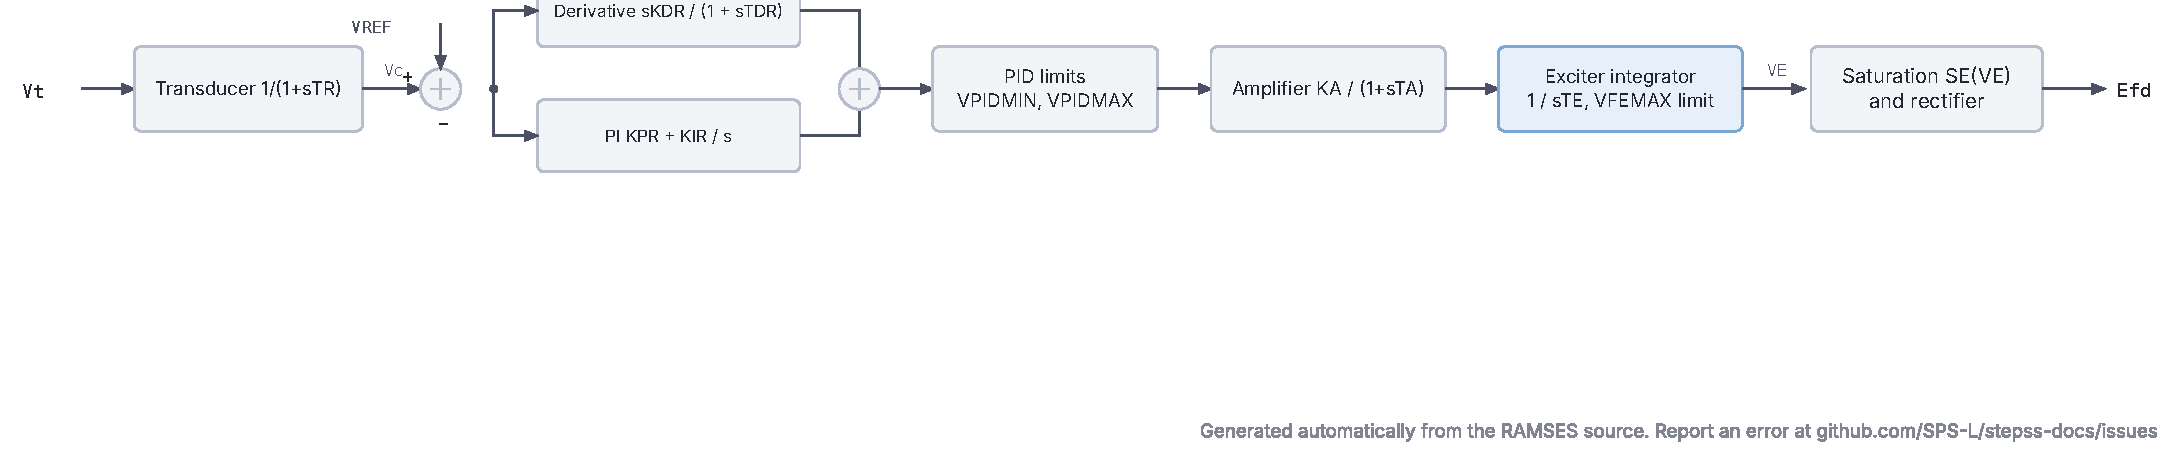
\includegraphics[width=0.98\linewidth]{figures/exc-ac8b-light}
\caption{AC8B block diagram.}
\end{figure}

\subsection{Mathematical Description}\label{model-exc-ieee-acdc:mathematical-description-2}

The PID voltage regulator:

\[\Delta V = V_c - V_{REF}\]

\[V_{PID}(s) = K_{PR} \cdot \Delta V + \frac{K_{IR}}{s} \cdot \Delta V + \frac{sK_{DR}/T_{DR}}{1 + sT_{DR}} \cdot \Delta V\]

\[V_R(s) = V_{PID} \cdot \frac{K_A}{1 + sT_A}, \quad V_{RMIN} \le V_R \le V_{RMAX}\]

The AC exciter with variable limits based on maximum field excitation voltage \(V_{FEMAX}\):

\[V_{FE} = K_D \cdot I_{fd} + \left(K_E + S_E(V_E)\right) V_E\]

\[\dot{V}_E = \frac{1}{T_E}(V_R - V_{FE}), \quad V_{EMIN} \le V_E \le \frac{V_{FEMAX} - K_D I_{fd}}{K_E + S_E(V_E)}\]

\subsection{Signal Flow}\label{model-exc-ieee-acdc:signal-flow-2}

\begin{enumerate}
\def\labelenumi{\arabic{enumi}.}
\tightlist
\item
  \textbf{Voltage measurement} (\texttt{tf1p}): \(V_c\) with \(T_R\)
\item
  \textbf{Error signal} (\texttt{algeq}): \(\Delta V = V_c - V_{REF}\)
\item
  \textbf{PID derivative part} (\texttt{tfder1p}): \(x_{der} \leftarrow \Delta V\) with gain \(K_{DR}/T_{DR}\)
\item
  \textbf{PID proportional-integral} (\texttt{pictl}): \(x_{propint} \leftarrow \Delta V\) with \(K_{IR}\), \(K_{PR}\)
\item
  \textbf{PID sum} (\texttt{algeq}): \(x_{pid} = x_{propint} + x_{der}\), limited to \([V_{PIDMIN}, V_{PIDMAX}]\)
\item
  \textbf{Amplifier} (\texttt{tf1plim}): \(V_R \leftarrow x_{pid}\) with \(K_A\), \(T_A\)
\item
  \textbf{Exciter integrator} (\texttt{invlim}): \(V_E\) with variable limits from \(V_{FEMAX}\)
\item
  \textbf{Saturation and rectification} (\texttt{algeq}): \(V_{FE}\), \(E_{fd}\)
\end{enumerate}

\subsection{Parameters}\label{model-exc-ieee-acdc:parameters-2}

\begin{small}\begin{longtable}[]{@{}lll@{}}
\toprule\noalign{}
Parameter & Description & Unit/Type \\
\midrule\noalign{}
\endhead
\bottomrule\noalign{}
\endlastfoot
\texttt{Kv} & Voltage compensation gain & pu \\
\texttt{Rc} & Line drop resistance & pu \\
\texttt{Xc} & Line drop reactance & pu \\
\texttt{TR} & Measurement time constant & s \\
\texttt{KPR} & PID proportional gain & pu \\
\texttt{KIR} & PID integral gain & pu/s \\
\texttt{KDR} & PID derivative gain & pu\ensuremath{\cdot}s \\
\texttt{TDR} & PID derivative filter time constant & s \\
\texttt{VPIDMAX} & PID output upper limit & pu \\
\texttt{VPIDMIN} & PID output lower limit & pu \\
\texttt{KA} & Amplifier gain & pu \\
\texttt{TA} & Amplifier time constant & s \\
\texttt{VRMAX} & Maximum regulator output & pu \\
\texttt{VRMIN} & Minimum regulator output & pu \\
\texttt{KC} & Rectifier commutation factor & pu \\
\texttt{KD} & Demagnetization factor & pu \\
\texttt{KE} & Exciter self-excitation constant & pu \\
\texttt{TE} & Exciter time constant & s \\
\texttt{VFEMAX} & Maximum field excitation voltage & pu \\
\texttt{VEMIN} & Minimum exciter output & pu \\
\texttt{VE1} & Saturation voltage point 1 & pu \\
\texttt{SE1} & Saturation factor at \(V_{E1}\) & pu \\
\texttt{VE2} & Saturation voltage point 2 & pu \\
\texttt{SE2} & Saturation factor at \(V_{E2}\) & pu \\
\end{longtable}\end{small}

\subsection{Variants}\label{model-exc-ieee-acdc:variants-2}

\begin{small}\begin{longtable}[]{@{}
  >{\raggedright\arraybackslash}p{(\linewidth - 4\tabcolsep) * \real{0.3097}}
  >{\raggedright\arraybackslash}p{(\linewidth - 4\tabcolsep) * \real{0.6903}}
@{}}
\toprule\noalign{}
\begin{minipage}[b]{\linewidth}\raggedright
Model
\end{minipage} & \begin{minipage}[b]{\linewidth}\raggedright
Description
\end{minipage} \\
\midrule\noalign{}
\endhead
\bottomrule\noalign{}
\endlastfoot
\texttt{AC8B} & Base model, IEEE Type AC8B \\
\texttt{AC8B\_PSS3B\_lim} & Adds PSS3B dual-input stabilizer and integral OEL + SCL (stator current limiter) \\
\texttt{AC8B\_lim} & Adds integral OEL and SCL without PSS \\
\end{longtable}\end{small}

\subsection{Usage Example}\label{model-exc-ieee-acdc:usage-example-2}

\begin{Verbatim}
SYNC_MACH  g1  g1
      # FP FQ P Q: share of the power-flow injection (FP, FQ) or initial power (P in MW, Q in Mvar)
      1.  1.  0.  0.
      # SNOM: Nominal apparent power, used as base power in the machine model (MVA)
      800.
      # Pnom: Nominal active power of the turbine, used as base power for the turbine model (MW)
      760.
      # H: Inertia constant (s)
      3.
      # D: Damping coefficient (usually set to zero when the damper windings are modelled) (pu)
      0.
      # IBRATIO: Field current base ratio I_fB^mac/I_fB^exc (see above) (pu)
      0.95
      # TYPE_MOD: Parameter format keyword: RL or XT (case-insensitive)
      XT
      # Xl: Leakage reactance L_l (pu)
      0.15
      # Xd: d-axis synchronous reactance (pu)
      1.1
      # X'd: d-axis transient reactance (must be smaller than Xd) (pu)
      0.25
      # X"d: d-axis subtransient reactance (pu)
      0.2
      # Xq: q-axis synchronous reactance (pu)
      0.7
      # X'q: q-axis transient reactance (pu)
      *
      # X"q: q-axis subtransient reactance (pu)
      0.2
      # m: Saturation coefficient (set to 0 to neglect saturation)
      0.1
      # n: Saturation exponent (ignored when m = 0)
      6.0257
      # Ra: Armature resistance (pu)
      0.
      # T'do: d-axis open-circuit transient time constant (s)
      5.00
      # T"do: d-axis open-circuit subtransient time constant (s)
      0.05
      # T'qo: q-axis open-circuit transient time constant (s)
      *
      # T"qo: q-axis open-circuit subtransient time constant (s)
      0.1
EXC  AC8B
      # Kv: weight of the terminal voltage in the measured voltage |Kv V + (Rc+jXc) I|; 1 = terminal voltage
      1.
      # Rc: Line drop resistance
      0.
      # Xc: Line drop reactance
      0.
      # TR: Measurement time constant
      0.02
      # KPR: PID proportional gain
      1.0
      # KIR: PID integral gain
      5.0
      # KDR: PID derivative gain
      0.1
      # TDR: PID derivative filter time constant
      0.1
      # VPIDMAX: RAMSES 3.84 applies this value as the LOWER limit of the PID output (pu)
      -8.0
      # VPIDMIN: RAMSES 3.84 applies this value as the UPPER limit of the PID output (pu)
      8.0
      # KA: Amplifier gain
      1.0
      # TA: Amplifier time constant
      0.1
      # VRMAX: Maximum regulator output
      6.5
      # VRMIN: Minimum regulator output
      -6.5
      # KC: Rectifier commutation factor
      0.2
      # KD: Demagnetization factor
      1.0
      # KE: Exciter self-excitation constant
      1.0
      # TE: Exciter time constant
      0.5
      # VFEMAX: Maximum field excitation voltage
      6.5
      # VEMIN: Minimum exciter output
      0.0
      # VE1: Saturation voltage point 1
      4.0
      # SE1: Saturation factor at V_E1
      0.3
      # VE2: Saturation voltage point 2
      3.0
      # SE2: Saturation factor at V_E2
      0.1
TOR  CONSTANT
;
\end{Verbatim}

\begin{center}\rule{0.5\linewidth}{0.5pt}\end{center}

\section{DC3A}\label{model-exc-ieee-acdc:dc3a}

The DC3A represents a non-continuously acting (rheostat-type) DC excitation system. It corresponds to IEEE Std 421.5-2016 Type DC3A. Rather than a proportional amplifier, it uses a three-position switch (VRMIN / VRH / VRMAX) driven by an integrator that holds the rheostat position \(V_{RH}\). The switch position is determined by whether the error signal \(V_{ERR}\) falls inside or outside a deadband \(\pm K_V\).

\begin{figure}[htbp]
\centering
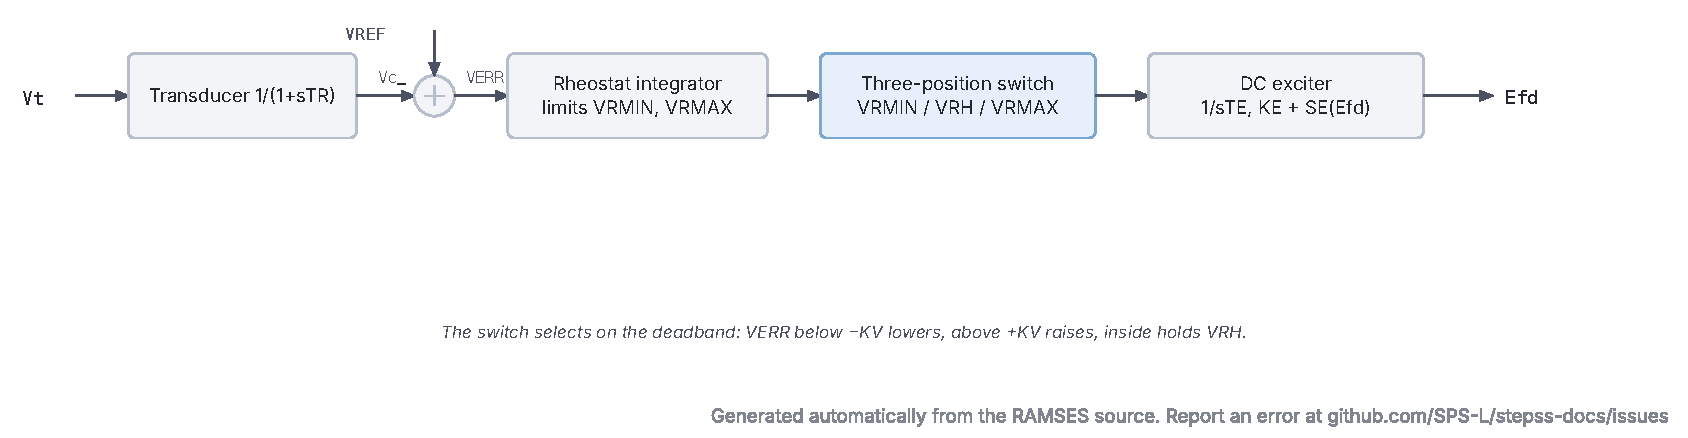
\includegraphics[width=0.98\linewidth]{figures/exc-dc3a-light}
\caption{DC3A block diagram.}
\end{figure}

\subsection{Mathematical Description}\label{model-exc-ieee-acdc:mathematical-description-3}

\[V_{ERR} = V_{REF} - V_c\]

The rheostat integrator:

\[\dot{V}_{RH} = \frac{K_V \cdot T_{RH}}{V_{RMAX} - V_{RMIN}} \cdot \text{clamp}(V_{ERR}, -K_V, K_V), \quad V_{RMIN} \le V_{RH} \le V_{RMAX}\]

The three-position switch:

\[V_R = \begin{cases} V_{RMIN} & V_{ERR} < -K_V \\ V_{RH} & |V_{ERR}| \le K_V \\ V_{RMAX} & V_{ERR} > K_V \end{cases}\]

The DC exciter with saturation:

\[\dot{E}_{fd} = \frac{1}{T_E}\left[V_R - \left(K_E + S_E(E_{fd})\right) E_{fd}\right]\]

\subsection{Parameters}\label{model-exc-ieee-acdc:parameters-3}

\begin{small}\begin{longtable}[]{@{}lll@{}}
\toprule\noalign{}
Parameter & Description & Unit/Type \\
\midrule\noalign{}
\endhead
\bottomrule\noalign{}
\endlastfoot
\texttt{Kvcomp} & Voltage compensation gain & pu \\
\texttt{Rc} & Line drop resistance & pu \\
\texttt{Xc} & Line drop reactance & pu \\
\texttt{TR} & Measurement time constant & s \\
\texttt{TRH} & Rheostat traversal time & s \\
\texttt{KV} & Sensitivity of non-continuously acting controller & pu \\
\texttt{VRMAX} & Maximum field voltage & pu \\
\texttt{VRMIN} & Minimum field voltage & pu \\
\texttt{TE} & Exciter time constant & s \\
\texttt{KE} & Exciter self-excitation constant & pu \\
\texttt{E1} & Saturation voltage point 1 & pu \\
\texttt{SE1} & Saturation factor at \(E_1\) & pu \\
\texttt{E2} & Saturation voltage point 2 & pu \\
\texttt{SE2} & Saturation factor at \(E_2\) & pu \\
\end{longtable}\end{small}

\subsection{Variants}\label{model-exc-ieee-acdc:variants-3}

\begin{small}\begin{longtable}[]{@{}
  >{\raggedright\arraybackslash}p{(\linewidth - 4\tabcolsep) * \real{0.2489}}
  >{\raggedright\arraybackslash}p{(\linewidth - 4\tabcolsep) * \real{0.7511}}
@{}}
\toprule\noalign{}
\begin{minipage}[b]{\linewidth}\raggedright
Model
\end{minipage} & \begin{minipage}[b]{\linewidth}\raggedright
Description
\end{minipage} \\
\midrule\noalign{}
\endhead
\bottomrule\noalign{}
\endlastfoot
\texttt{DC3A} & Base model, IEEE Type DC3A, non-continuously acting rheostat controller \\
\end{longtable}\end{small}

\subsection{Usage Example}\label{model-exc-ieee-acdc:usage-example-3}

\begin{Verbatim}
SYNC_MACH  g1  g1
      # FP FQ P Q: share of the power-flow injection (FP, FQ) or initial power (P in MW, Q in Mvar)
      1.  1.  0.  0.
      # SNOM: Nominal apparent power, used as base power in the machine model (MVA)
      800.
      # Pnom: Nominal active power of the turbine, used as base power for the turbine model (MW)
      760.
      # H: Inertia constant (s)
      3.
      # D: Damping coefficient (usually set to zero when the damper windings are modelled) (pu)
      0.
      # IBRATIO: Field current base ratio I_fB^mac/I_fB^exc (see above) (pu)
      0.95
      # TYPE_MOD: Parameter format keyword: RL or XT (case-insensitive)
      XT
      # Xl: Leakage reactance L_l (pu)
      0.15
      # Xd: d-axis synchronous reactance (pu)
      1.1
      # X'd: d-axis transient reactance (must be smaller than Xd) (pu)
      0.25
      # X"d: d-axis subtransient reactance (pu)
      0.2
      # Xq: q-axis synchronous reactance (pu)
      0.7
      # X'q: q-axis transient reactance (pu)
      *
      # X"q: q-axis subtransient reactance (pu)
      0.2
      # m: Saturation coefficient (set to 0 to neglect saturation)
      0.1
      # n: Saturation exponent (ignored when m = 0)
      6.0257
      # Ra: Armature resistance (pu)
      0.
      # T'do: d-axis open-circuit transient time constant (s)
      5.00
      # T"do: d-axis open-circuit subtransient time constant (s)
      0.05
      # T'qo: q-axis open-circuit transient time constant (s)
      *
      # T"qo: q-axis open-circuit subtransient time constant (s)
      0.1
EXC  DC3A
      # Kvcomp: weight of the terminal voltage in the measured voltage |Kv V + (Rc+jXc) I|; 1 = terminal voltage
      1.
      # Rc: Line drop resistance
      0.
      # Xc: Line drop reactance
      0.
      # TR: Measurement time constant
      0.0
      # TRH: Rheostat traversal time
      1.0
      # KV: voltage error band; beyond +/-KV the output is forced to VRMAX or VRMIN (pu)
      0.05
      # VRMAX: upper limit of the rheostat output, also the forced value when the error exceeds KV (pu)
      5.0
      # VRMIN: lower limit of the rheostat output, also the forced value when the error is below -KV (pu)
      0.0
      # TE: Exciter time constant
      0.8
      # KE: Exciter self-excitation constant
      1.0
      # E1: Saturation voltage point 1
      3.1
      # SE1: Saturation factor at E_1
      0.33
      # E2: Saturation voltage point 2
      2.3
      # SE2: Saturation factor at E_2
      0.1
TOR  CONSTANT
;
\end{Verbatim}
